\section{Literature Review}\label{sec-comprehend}
%\yanyan{I feel this section still belongs to intro. You could cut
%these sentences and place them in appropriate places in intro
%where you need more supporting evidence.}
Code comprehension is the process by which a developer creates a 
mental model of a software system’s architecture, 
behaviors, and actions based upon the source code. With the increase of more developers on projects, the need
for a uniform understanding of the source between developers is key to the successful development of
software.
As code comprehension is such a vital area for moving forward in 
a software development life-cycle, then it stands to reason that 
making comprehension a more natural process by improving upon the source code is a worthwhile endeavor.

Just during maintenance and re-factoring stages developers spend a major 
portion of their time, approximately 60-90\%~\cite{ward_program_nodate}, on simply trying to understand the
source code. In fact many development teams would
benefit greatly, reducing a significant portion of the 
maintenance and re-factoring overhead by simply making their 
software easier to comprehend. 

\begin{figure*}%[ht]
\centering
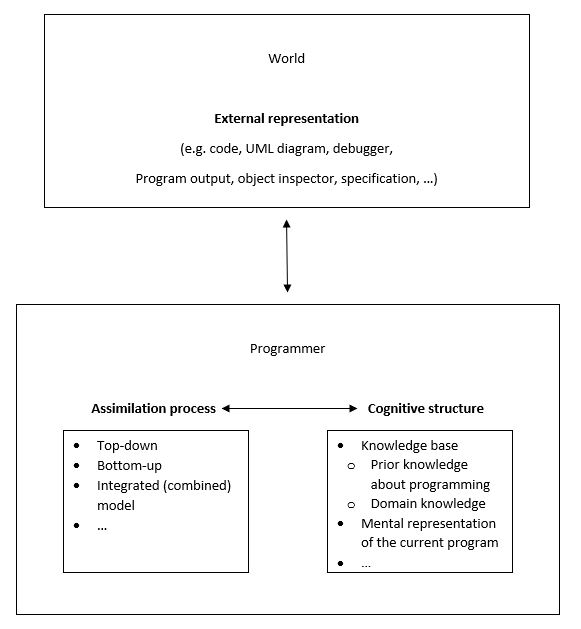
\includegraphics[scale=0.85]{images/ProgramCompModels}
\caption{Commonalities in comprehension models.} 
\label{fig:models}
\end{figure*}

Software maintenance is a very costly, broad, and complicated process 
as it requires very deep understanding of the target system source 
code. Moreover, professional
developers must be familiar with the system undergoing change in order to accomplish
the required maintenance tasks \cite{alhindawi_degree_nodate}. 
\yanyan{This paragraph lacks some logic. What's the purpose? Should
some of these sentences be spread out in other paragraphs as 
examples or supporting evidence?}

